\documentclass[aps,pra,twocolumn,superscriptaddress,floatfix,nofootinbib]{revtex4-2}

\usepackage{graphicx}
\usepackage{amsmath,amssymb}
\usepackage{booktabs}
\usepackage[colorlinks=true,linkcolor=blue,citecolor=blue,urlcolor=blue]{hyperref}

\graphicspath{{../figures/}}

\begin{document}

\title{Iterate, sample, evolve: three ways of teaching a computer to do physics.\\
Notes from an undergraduate computational-physics course}

\author{Tien D. Nguyen}
\affiliation{Faculty of Physics, Hanoi University of Science, VNU Hanoi, 120401 Vietnam}

\date{\today}

\begin{abstract}
This note accompanies a small repository of code written by hand during an undergraduate course in computational physics. It is an undergraduate project and is kept for no other reason than that it is, most probably, the last code its author wrote line by line. Course materials/problems are from HUS's undergraduate physics courses PHY3502/3508 Computational Physics I and II. The exercises are simple, but they are very representative, in the sense that they illustrate what it means for a computer to ``solve'' a physics problem. In the first part the computer \emph{iterates}: a system of two nonlinear equations is solved by Newton--Raphson with a hand-derived Jacobian and the eigenvalues of a $5\times5$ matrix are extracted by unshifted QR iteration. In the second part it \emph{samples}: the $\pi$ number, integrals and the survival of a population of radioactive nuclei are obtained from random numbers, which prompts the question of where those numbers come from (linear congruential generator, Box--Muller, rejection sampling) and how large the resulting errors are; the part closes with Bateman decay chains and a branching chain $^{211}\mathrm{Rn}\to\cdots\to{}^{207}\mathrm{Pb}$. In the third part it \emph{evolves}: a box of free-flying molecules is followed collision by collision to read off a pressure, and the one-dimensional heat equation is integrated with forward Euler, backward Euler and Crank--Nicolson. Some human failures were revisited by Claude in the Conclusion with some comments, comments that highlight the cold hard truth surfacing omniously these days: the capabilities of AI has superseded that of human in numerous areas. From here onward, everything is AI-generated.  
\end{abstract}

\maketitle

\section{Introduction}
\label{sec:intro}

A computational-physics course is usually the first place where a physics student meets the three habits that later become second nature: writing an equation in a form a machine can iterate, replacing an integral by an average over random numbers, and replacing a derivative by a difference. The material collected in the accompanying repository~\footnote{The repository layout is summarised in Appendix~\ref{app:repo}.} was produced for the midterm and final assignments of one such course and has no scientific novelty. It is published for a personal reason: it was written entirely by hand, line by line, at a moment just before code-generating tools made that practice optional. The author expects it to be the last substantial piece of code written this way, and keeps it as one keeps a lab notebook.

The exercises were set as independent problems, but they fall naturally into three acts that this note uses as its story line. In Sec.~\ref{sec:iterate} the computer is asked to \emph{iterate}: starting from a guess it repeats a deterministic update until a residual drops below a tolerance. In Sec.~\ref{sec:sample} it is asked to \emph{sample}: the answer is an expectation value, and the computer earns it by drawing random numbers. In Sec.~\ref{sec:evolve} it is asked to \emph{evolve}: a physical state is pushed forward in time, either event by event or on a grid. Each act ends with something that did not work, and Sec.~\ref{sec:outlook} explains why, because the failures taught more than the successes. All numbers quoted below are read directly from the stored notebook outputs; nothing was re-run for this note. The original notebooks are kept untouched in the repository's \texttt{misc/} folder.

\section{Act I: Iterate}
\label{sec:iterate}

\subsection{Roots of a nonlinear system}

The first problem asks for all solutions of
\begin{align}
\cos(xy) + \sin(x^4+y^4) &= 1, \nonumber\\
x^2 + y^2 + \sin(xy) &= 3
\label{eq:system}
\end{align}
inside the square $-2\le x,y\le 2$, together with an estimate of their absolute error. The approach is the textbook one~\cite{Ypma1995,NumericalRecipes2007}: locate the roots graphically, then polish each one by Newton--Raphson.

Figure~\ref{fig:contours} shows the zero-level sets of the two residuals on a $600\times600$ grid. The second equation is a slightly deformed circle of radius $\sqrt3$; the first is a far wilder curve, because $\sin(x^4+y^4)$ oscillates ever faster away from the origin. Where the blue and red curves cross, Eq.~\eqref{eq:system} has a solution, and twelve crossings can be read off inside the square by eye. These became the twelve initial guesses, for instance $(1.224, 0.815)$ and $(1.752, -0.072)$.

\begin{figure}[tb]
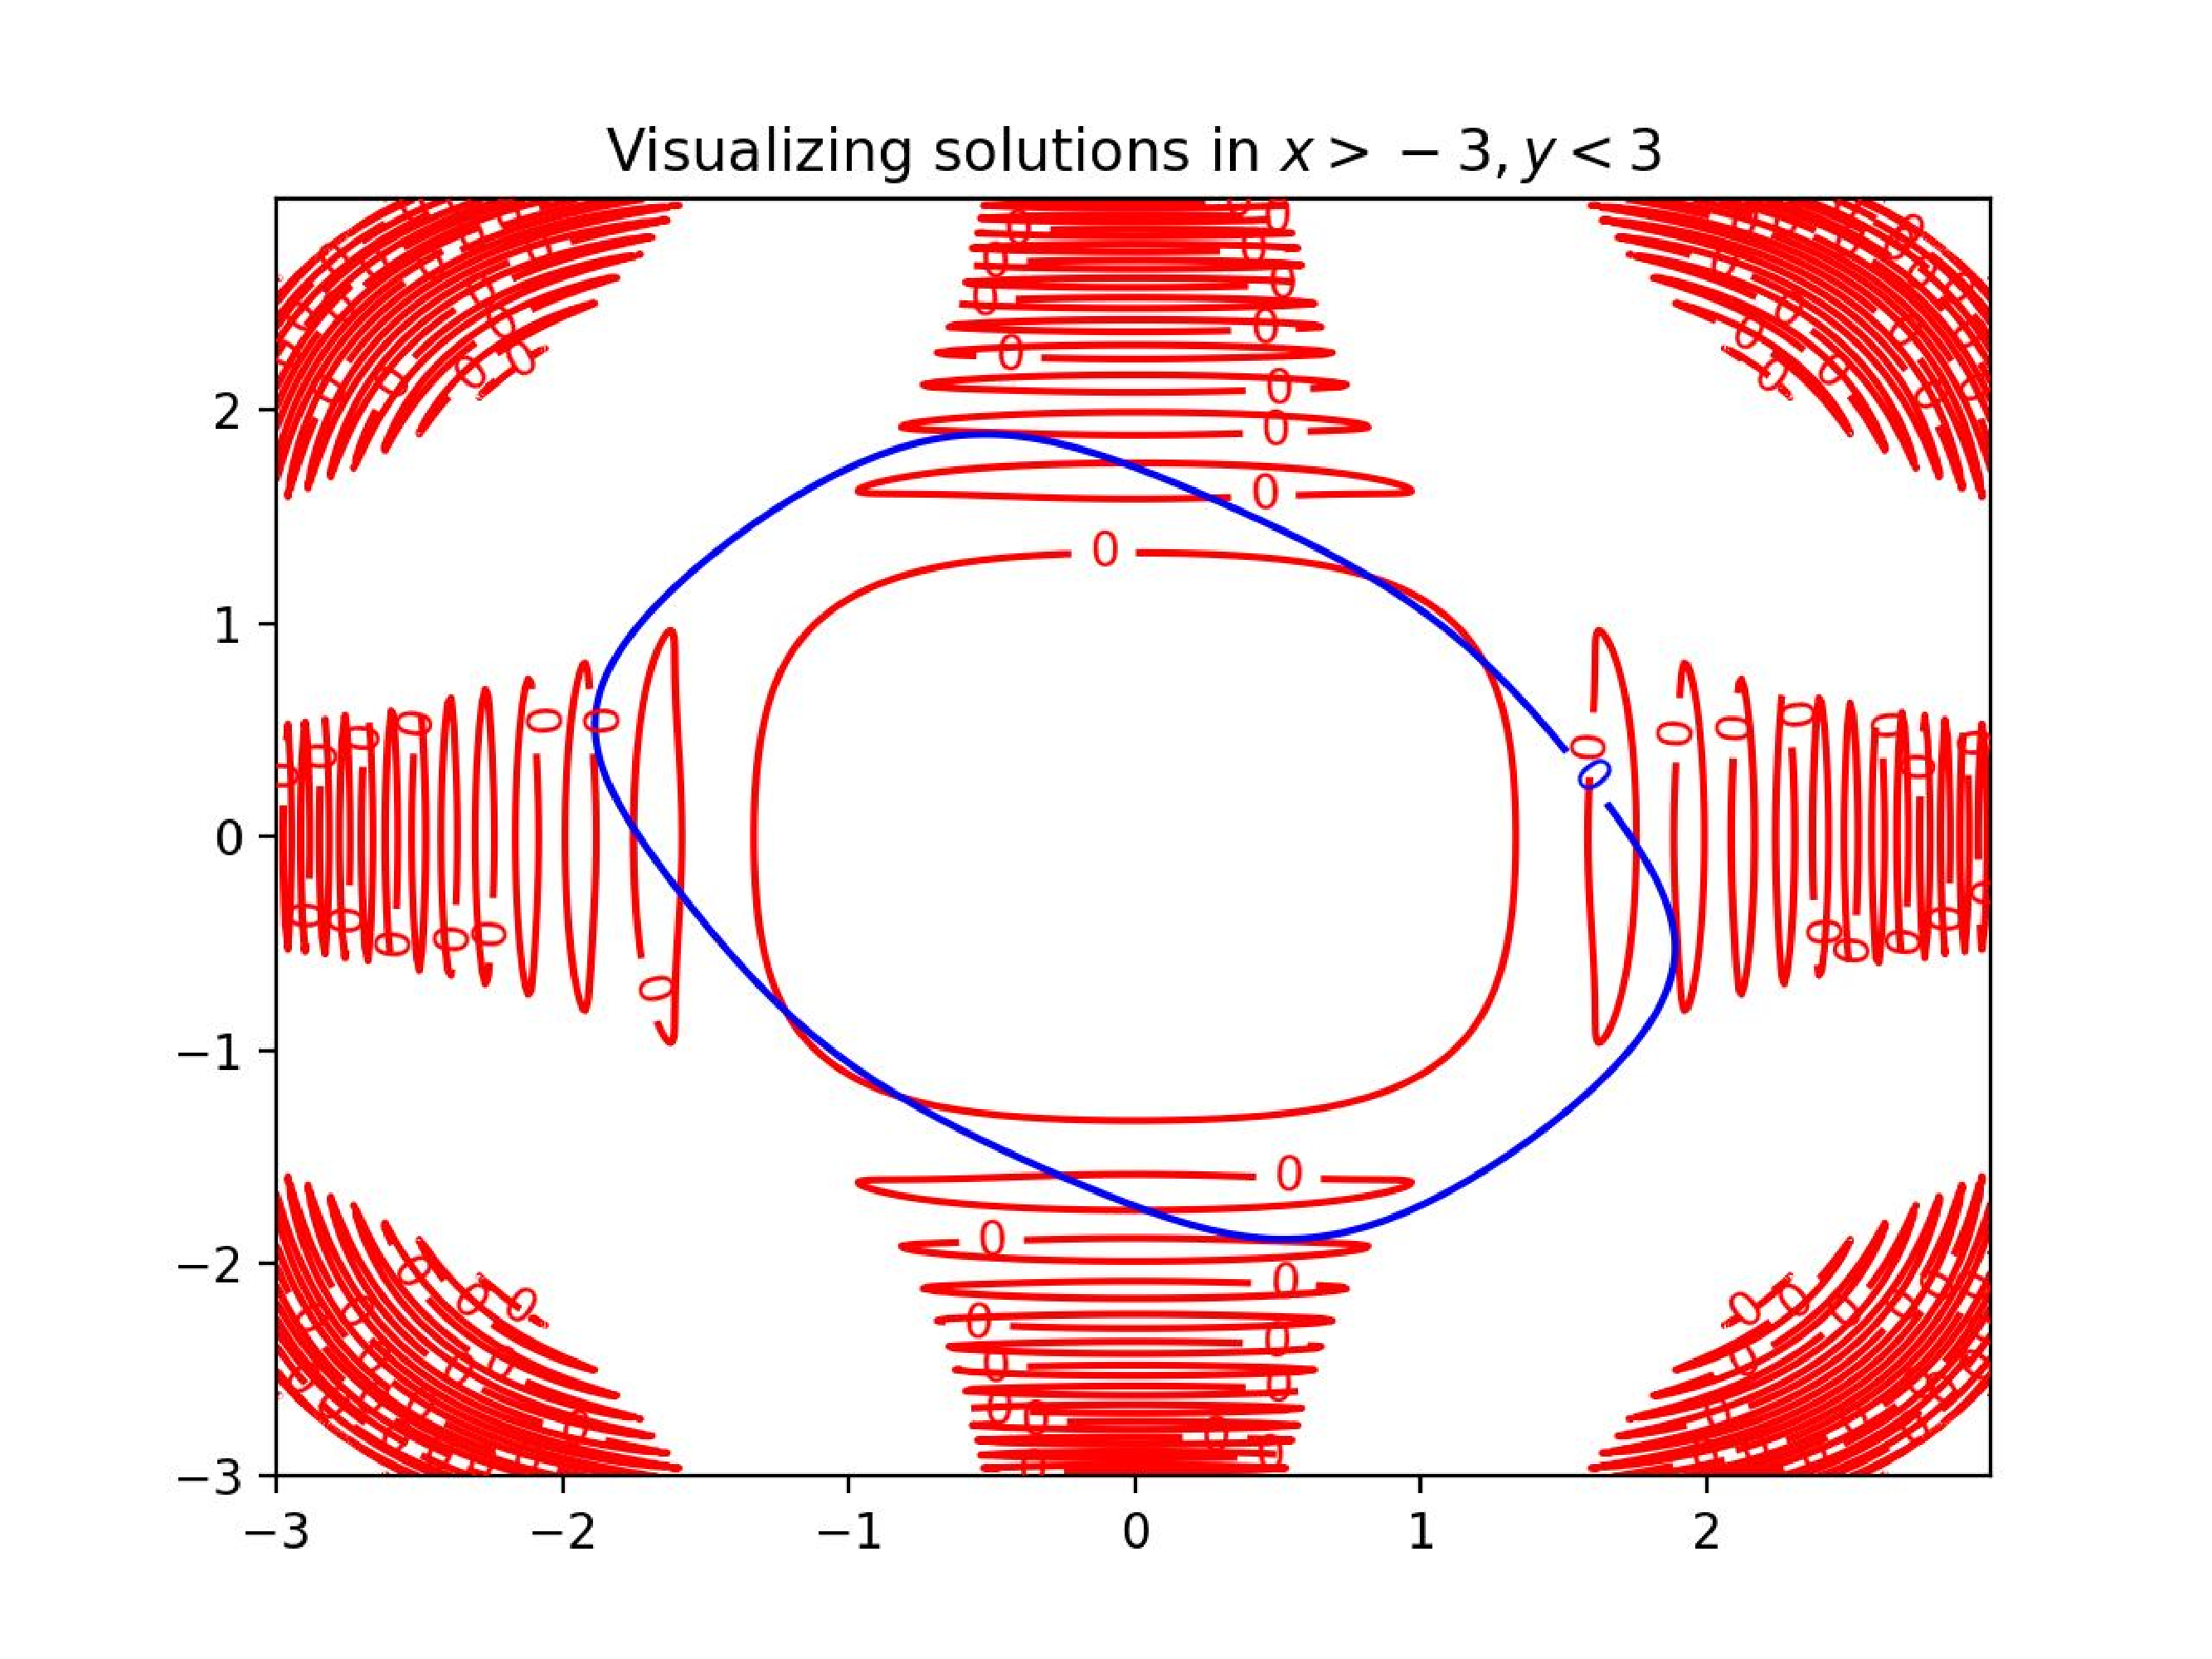
\includegraphics[width=\columnwidth]{01_nonlinear_system_zero_contours}
\caption{Zero-level sets of the two residuals of Eq.~\eqref{eq:system}: $\cos(xy)+\sin(x^4+y^4)-1$ in red and $x^2+y^2+\sin(xy)-3$ in blue. Each crossing is a solution; the twelve crossings inside $-2\le x,y\le2$ were used as starting points for Newton--Raphson.}
\label{fig:contours}
\end{figure}

Newton's step solves $J(\mathbf x_n)\,\boldsymbol\Delta = -\mathbf F(\mathbf x_n)$ and sets $\mathbf x_{n+1}=\mathbf x_n+\boldsymbol\Delta$. The $2\times2$ Jacobian was derived symbolically with \textsc{sympy} and then transcribed into a plain \textsc{numpy} function. The inner linear solve was first written as a Gauss--Seidel iteration~\cite{Saad2003}, which was validated on a $3\times3$ test system against \texttt{numpy.linalg.solve} (both give $(1.025, 1.175, 2.225)$), and then, for simplicity, the built-in solver was used in the Newton loop while the home-made one was left in as a comment. The stopping criterion is $\lVert\mathbf F(\mathbf x)\rVert_2<10^{-10}$ and the absolute error is reported as $\lVert\boldsymbol\Delta\rVert_2/\lVert\mathbf x\rVert_2$ at each step.

The behaviour is textbook quadratic convergence. From $(1.752,-0.072)$ the reported errors are $1.8\times10^{-2}$, $3.2\times10^{-4}$ and $1.0\times10^{-7}$ on three successive iterations, and the solver stops at $(1.75201771,\,-0.04068550)$. Most of the twelve guesses converge in three steps; the guess $(0.265, 1.500)$, which lies on a flatter part of the red curve, needs seven, its error creeping down through $0.16$, $0.13$, $0.11$, $0.058$, $0.0087$ before collapsing to $3\times10^{-9}$. A reader who has only ever called a library root-finder will find it instructive to watch the exponent double.

\subsection{Eigenvalues by QR iteration}

The second problem asks for at least three eigenvalues and eigenvectors of
\begin{equation}
A=\begin{pmatrix}
1&1&1&2&3\\ 2&3&2&1&2\\ 1&2&2&1&1\\ 1&2&0&4&1\\ 2&2&1&4&6
\end{pmatrix},
\label{eq:A}
\end{equation}
by a numerical method, and for a discussion of its merits. The method chosen is the unshifted QR iteration~\cite{Francis1961,Francis1962,GolubVanLoan2013}: factor $A_k=Q_kR_k$, form $A_{k+1}=R_kQ_k=Q_k^{\!\top}A_kQ_k$, and repeat. Each step is a similarity transformation, so the spectrum is preserved, and for a matrix with eigenvalues of distinct modulus the sequence converges to an upper-triangular matrix with the eigenvalues on the diagonal.

Two details are worth recording because they were the author's own. First, the stopping rule: every five iterations the number of entries below $10^{-4}$ in modulus is counted, and the loop stops when that count has stopped growing---a crude but effective way of detecting that the sub-diagonal has frozen. The run stopped after ten iterations. Second, $A$ is real but not symmetric, so it has complex eigenvalues; those cannot appear on the diagonal of a real matrix, and the iteration instead converges to a \emph{quasi}-triangular (real Schur) form with $2\times2$ blocks on the diagonal:
\begin{equation}
A_{10}\simeq\begin{pmatrix}
10.275&-0.765&2.240&-0.866&-0.345\\
0&2.737&1.186&-0.835&0.864\\
0&-0.484&2.434&-1.097&-1.199\\
0&0&0&0.224&0.801\\
0&0&0&-0.009&0.329
\end{pmatrix}.
\end{equation}
The code then scans the sub-diagonal for entries above $10^{-3}$, cuts out the corresponding $2\times2$ blocks, and solves their characteristic quadratics by hand. The result,
\begin{equation}
\lambda = 10.2754,\quad 2.5857\pm0.7421\,i,\quad 0.2765\pm0.0649\,i,
\end{equation}
agrees with \texttt{numpy.linalg.eigvals} to six figures in the dominant eigenvalue and to five in the complex pairs. The advantage of the method, in the author's words from the assignment, is that it finds all eigenvalues at once without forming the characteristic polynomial; the disadvantage is slow convergence of the unshifted variant, and the need for the quasi-triangular bookkeeping when the matrix is not symmetric.

The eigenvector part is the first instructive failure. For the dominant eigenvalue the code forms $\tilde A = A-\lambda_1 I$ and tries to solve $\tilde A\mathbf v=\mathbf 0$ with the Gauss--Seidel routine from Problem~1, starting from $\mathbf v=\mathbf 0$. The answer is, of course, $\mathbf v = \mathbf 0$: the zero vector is a fixed point of any homogeneous iteration, and \texttt{numpy.linalg.solve} returns the same trivial vector. The notebook ends on that honest line. What was missing is explained in Sec.~\ref{sec:outlook}.

\section{Act II: Sample}
\label{sec:sample}

The second act replaces the deterministic grid by random points. The notebook's own introduction is a paragraph lifted from Wikipedia ``to make the notebook less abrupt''; the content, however, is a sequence of small experiments that build on each other, and this section follows them in order.

\subsection{$\pi$, integrals, and a decaying population}

The simplest Monte-Carlo estimate~\cite{MetropolisUlam1949} throws $N_0$ points uniformly into the unit square and counts the fraction inside the quarter circle (``hit-or-miss''), or averages $\sqrt{1-x^2}$ over uniform $x$ (``sample mean''). With $N_0=10^5$ the two give $3.14432$ and $3.13954$, both within $10^{-3}$ of $\pi$, as expected for an error of order $N_0^{-1/2}$.

The same two estimators are then applied to definite integrals in one, two and three dimensions; the results, compared here with adaptive quadrature evaluated for this note, are collected in Table~\ref{tab:integrals}. Two patterns stand out. The sample-mean estimator is uniformly the better one, because hit-or-miss wastes most of its points when the integrand is small compared with the bounding box (the one-dimensional integrand stays below $0.1$ in magnitude while the box height is~1). And integrating over a non-rectangular region---a disk or a cylinder---costs nothing extra: points outside the region simply contribute zero, which is the first hint of why Monte Carlo wins in many dimensions.

\begin{table}[tb]
\caption{Monte-Carlo integrals from the notebook ($N=10^4$ points each) against adaptive quadrature, for
$f_1=\cos x/\sqrt{1+x^4}+0.05$,
$f_2=y^3e^y/(x^2+y^2)$ and
$f_3=[x^2+y^2+(z-2)^2]^{-1/2}$.
``sm'' and ``sp'' are the sample-mean estimator on a box and on a sub-region of it, ``hm'' is hit-or-miss. The box for $f_3$ is $[-1,1]\times[-\tfrac32,\tfrac32]\times[-1,1]$.}
\label{tab:integrals}
\footnotesize
\begin{ruledtabular}
\begin{tabular}{llcrr}
 & Region & Method & MC & Quad.\\
\colrule
$\int f_1\,dx$ & $[2,10]$ & sp & 0.2213 & 0.2249\\
 & & hm & 0.2080 & \\
$\iint f_2\,dx\,dy$ & $[1,2]\times[3,4]$ & sm & 104.85 & 104.91\\
 & & hm & 106.15 & \\
 & disk $(x-\tfrac12)^2+y^2<1$ & sp & 0.575 & 0.544\\
$\iiint f_3\,dV$ & box & sm & 5.660 & 5.647\\
 & cylinder $x^2+y^2\le1$ & sp & 3.169 & 3.172\\
\end{tabular}
\end{ruledtabular}
\end{table}

The physics enters with radioactive decay. Each of $N_0=10^5$ nuclei is a boolean; at every time step a uniform random number is drawn per nucleus and the nucleus survives if that number exceeds $p=\ln2/T_{1/2}$. Figure~\ref{fig:decay} compares the simulated survival with $N_0\,2^{-t/T_{1/2}}$ for $T_{1/2}=3.8$. The two curves have the same shape but the simulation lies visibly below the analytic law, and the gap is not statistical: with a time step equal to the unit of $T_{1/2}$ the survival factor per step is $1-p=0.818$ instead of $e^{-p}=0.833$, so after fifteen steps the simulation has lost about $25\%$ more nuclei than it should. The discrete-time Monte Carlo is exact only in the limit $p\,\Delta t\to0$; this is the same first-order error as a forward-Euler step, met here from the stochastic side.

\begin{figure}[tb]
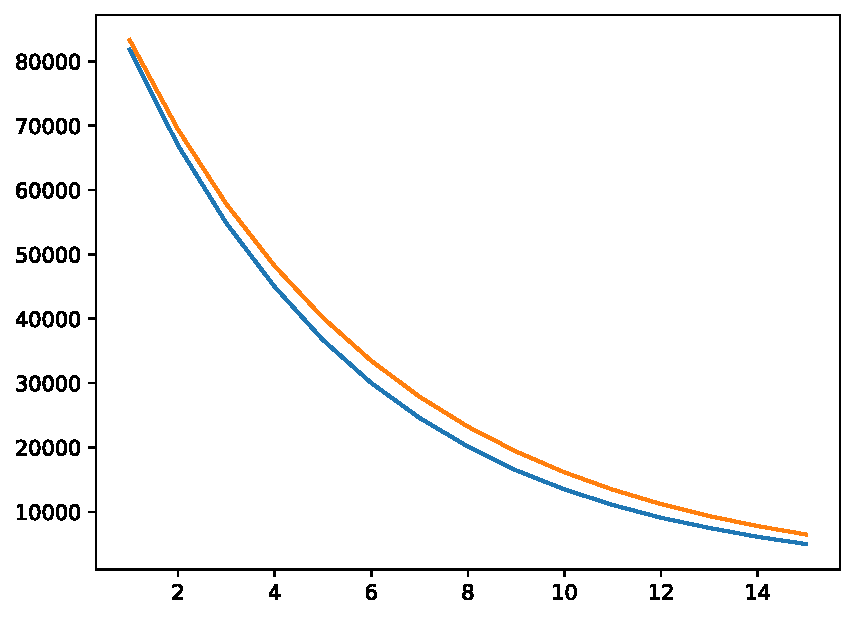
\includegraphics[width=\columnwidth]{02a_decay_mc_vs_analytic}
\caption{Survival of $10^5$ nuclei with $T_{1/2}=3.8$: Monte-Carlo population (blue) and the analytic law $N_0 2^{-t/T_{1/2}}$ (orange). The systematic offset is the discretisation error $(1-p)^t$ versus $e^{-pt}$ discussed in the text.}
\label{fig:decay}
\end{figure}

The notebook then sets out to ``prove'', in its own cautious words, that the number of decays in a unit interval is Poisson distributed: the one-step experiment is repeated $10^5$ times with $N_0=10^4$ nuclei and $p=\ln2/(3.8\times24)$, and the histogram of decay counts is overlaid with $e^{-\mu}\mu^k/k!$, $\mu=pN_0\simeq76$ (Fig.~\ref{fig:poisson}). The agreement is excellent, which is the computational counterpart of Rutherford and Geiger's 1910 experiment~\cite{RutherfordGeiger1910}.

\begin{figure}[tb]
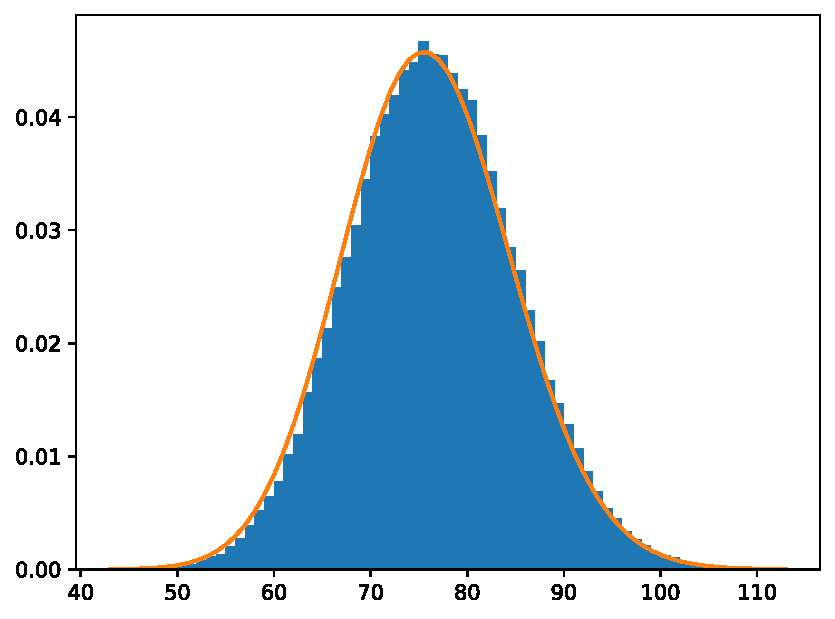
\includegraphics[width=\columnwidth]{02b_decay_counts_poisson}
\caption{Number of decays per unit time in $10^5$ repetitions of a one-step experiment on $10^4$ nuclei, with the Poisson mass function of mean $\mu=pN_0$ superimposed.}
\label{fig:poisson}
\end{figure}

\subsection{Where the random numbers come from}

Having used \texttt{numpy.random.uniform} freely, the second chapter asks what is behind it. A linear congruential generator $X_{n+1}=(aX_n+c)\bmod m$ with the Park--Miller ``minimal standard'' constants $a=16807$, $c=0$, $m=2^{31}-1$~\cite{ParkMiller1988} is written in five lines and its $10^4$ outputs, normalised by their maximum, fill ten histogram bins to within the expected $\sqrt{1000}\simeq30$ counts (Fig.~\ref{fig:rng}, left).

Uniform numbers are turned into Gaussian ones by the Box--Muller transform~\cite{BoxMuller1958}, $G_{1,2}=\sqrt{-2\ln U_1}\,\{\sin,\cos\}(2\pi U_2)$, fed with two LCG streams; the histograms of $G_1$ and $G_2$ against the standard normal are shown in Fig.~\ref{fig:rng}, right. (The density used for the overlay, as written in the notebook, has its $\sigma^2$ in the numerator of the exponent rather than the denominator; for $\sigma=1$ this is invisible, and the comparison is sound.)

\begin{figure}[tb]
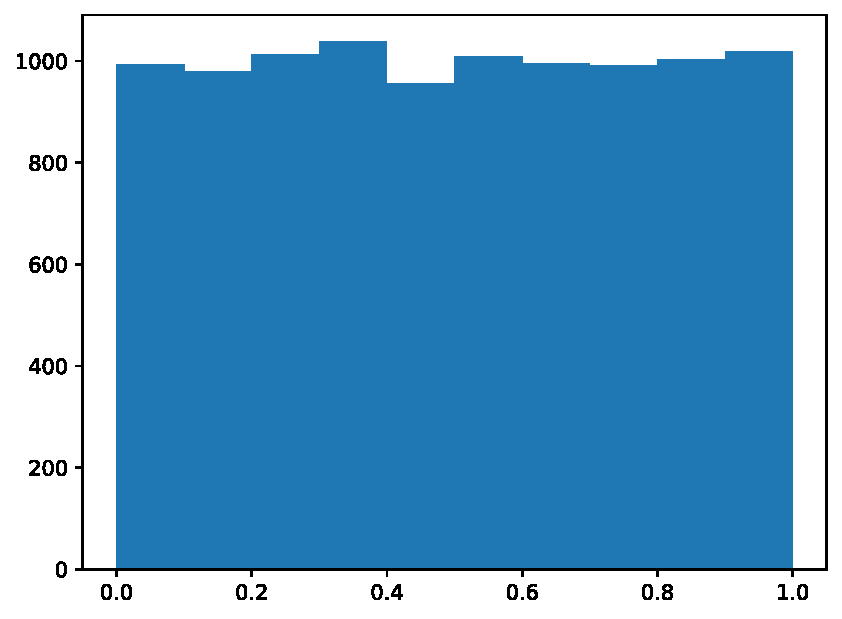
\includegraphics[width=0.48\columnwidth]{02c_lcg_uniform_histogram}\hfill
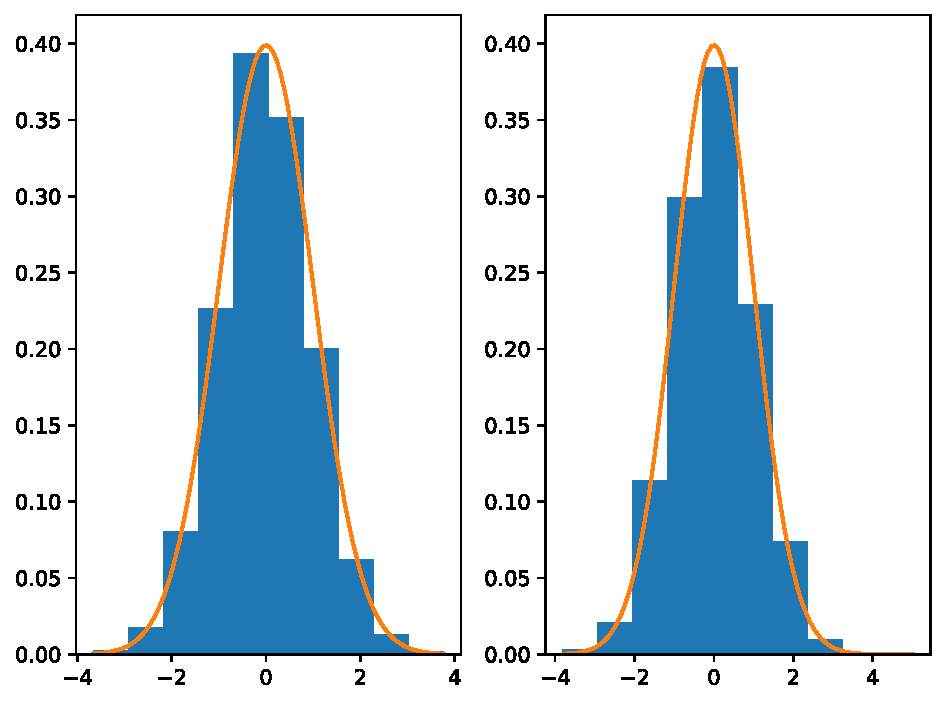
\includegraphics[width=0.48\columnwidth]{02d_box_muller_gaussians}
\caption{Left: $10^4$ numbers from the home-made linear congruential generator. Right: the two Box--Muller outputs built from them, against $N(0,1)$.}
\label{fig:rng}
\end{figure}

For an arbitrary target density the notebook turns to rejection sampling~\cite{vonNeumann1951}, and picks a deliberately ugly one, $\rho(x)=\tfrac23x^{-1/3}$, which diverges at the origin. The accompanying plot (Fig.~\ref{fig:rejection}, left) makes the difficulty visible: no finite envelope covers the spike, and the text concludes that a cut-off is needed, implementing $\rho(x)=15$ for $x<0.1$. The sampler that was finally written and run, however, targets the Maxwell--Boltzmann speed distribution
\begin{equation}
\rho_{\rm MB}(v)=\sqrt{\frac2\pi}\,\frac{v^2}{a^3}\,e^{-v^2/2a^2},
\end{equation}
with $a=2$: uniform proposals on $[0,20]$ are accepted when a second uniform number below $F_{\max}=0.3$ falls under the curve. The $10^5$ accepted speeds reproduce the density essentially perfectly (Fig.~\ref{fig:rejection}, right), which is the first genuinely physical distribution the course generates from scratch.

\begin{figure}[tb]
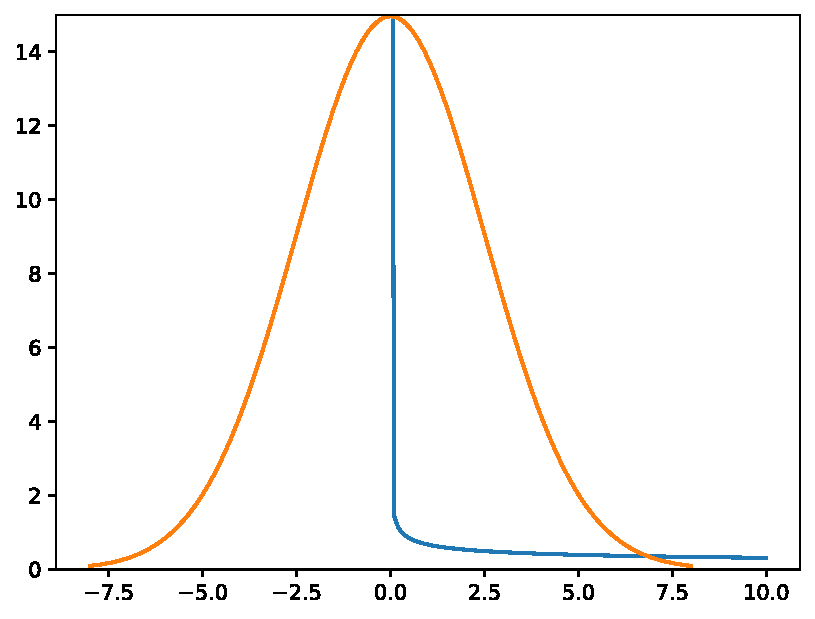
\includegraphics[width=0.48\columnwidth]{02e_rejection_target_vs_gaussian_envelope}\hfill
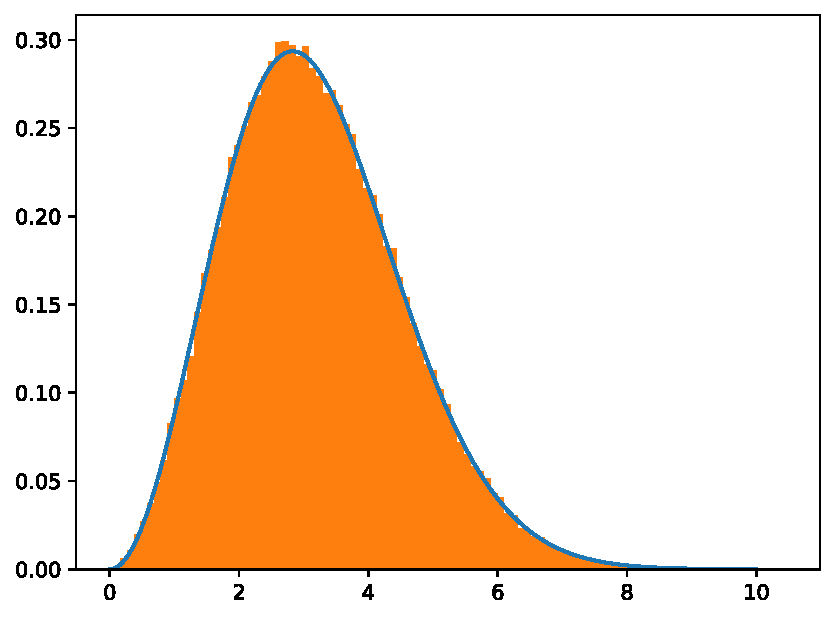
\includegraphics[width=0.48\columnwidth]{02g_maxwell_boltzmann_rejection_sampling}
\caption{Left: the divergent target $\tfrac23x^{-1/3}$ (blue) next to a scaled Gaussian (orange), illustrating why a cut-off is needed before rejection sampling. Right: $10^5$ speeds drawn by rejection sampling (orange histogram) against the Maxwell--Boltzmann density with $a=2$ (blue).}
\label{fig:rejection}
\end{figure}

\subsection{How wrong are we?}

A short third chapter pauses to ask, in the notebook's words, ``hmm okay what about the errors?'' The $\pi$ estimator is run $500$ times with only $N_0=1000$ points each and the spread of the results is computed from $\langle\pi^2\rangle-\langle\pi\rangle^2$. For hit-or-miss the expected standard deviation of a single run is $4\sqrt{p(1-p)/N_0}$ with $p=\pi/4$, i.e.\ $0.052$ at $N_0=1000$, falling as $N_0^{-1/2}$; the notebook's expression divides additionally by $\sqrt{499}$ and so reports the standard error of the mean of the $500$ runs, about $2\times10^{-3}$. The chapter closes with the remark that the same procedure applies to any Monte-Carlo program, which is the right lesson even if the quantity computed is not quite the one named.

\subsection{Chains of decays}

The climax of the second act returns to radioactivity with the Bateman equations~\cite{Bateman1910},
\begin{align}
\dot N_1 &= -\lambda_1N_1,\nonumber\\
\dot N_i &= -\lambda_iN_i+\lambda_{i-1}N_{i-1},\nonumber\\
\dot N_k &= +\lambda_{k-1}N_{k-1},
\end{align}
which can be solved in closed form for a short chain but, as the notebook notes, become unwieldy as the chain grows, whereas the Monte-Carlo program barely changes. Three boolean arrays now track which of $10^4$ nuclei is of species 1, 2 or 3; each step, species-1 nuclei that decay are moved into species 2 and species-2 nuclei that decay into species 3. With $T_{1/2}=14.8$ and $16.1$ the familiar picture emerges (Fig.~\ref{fig:bateman}): the parent decays exponentially, the daughter rises, peaks near $t\simeq22$ where $\lambda_1N_1=\lambda_2N_2$, and decays in turn while the stable granddaughter saturates. A side experiment repeats the Poisson test for the krypton parent and again recovers the Poisson curve (not shown; \texttt{figures/02i}).

\begin{figure}[tb]
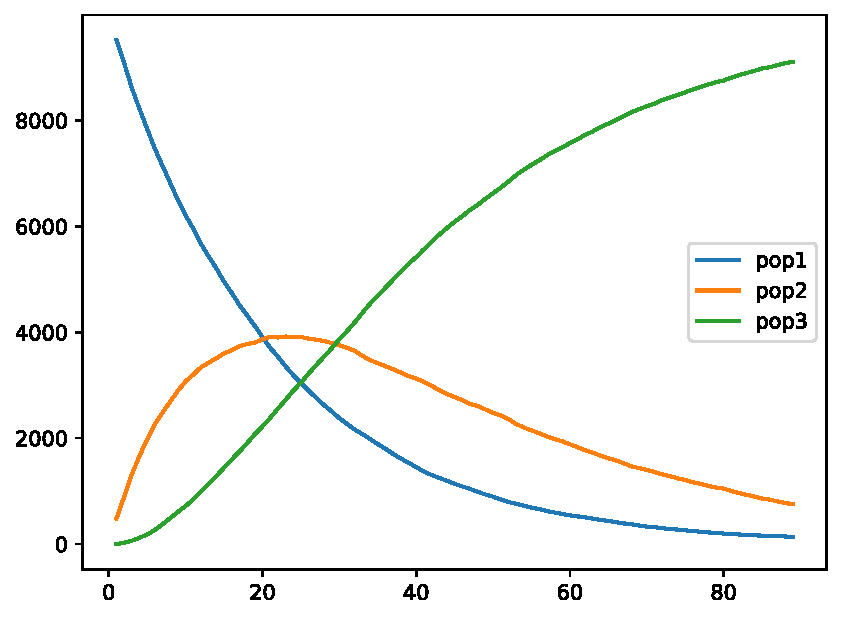
\includegraphics[width=\columnwidth]{02h_bateman_three_nuclei_chain}
\caption{Three-species Bateman chain simulated for $10^4$ nuclei with $T_{1/2}=14.8$ and $16.1$: parent (pop1), daughter (pop2) and stable granddaughter (pop3).}
\label{fig:bateman}
\end{figure}

The last and, in the author's words, ``pretty hard'' example adds branching. The chain modelled is
\begin{equation}
{}^{211}\mathrm{Rn}\;
\begin{cases}
\xrightarrow{74\%}\;{}^{211}\mathrm{At}\to{}^{211}\mathrm{Po}\to{}^{207}\mathrm{Pb}\\[2pt]
\xrightarrow{26\%}\;{}^{207}\mathrm{Po}\to{}^{207}\mathrm{Bi}\to{}^{207}\mathrm{Pb}
\end{cases}
\end{equation}
with half-lives of $15$, $7.2$ and $5.7$~h for Rn, At and Po-207, a $^{211}$Po that decays essentially within one step ($\lambda=0.99999\,\mathrm h^{-1}$) and a $^{207}$Bi that is essentially stable on the $200$~h window ($\lambda=10^{-5}\,\mathrm h^{-1}$). Six boolean arrays and four streams of random numbers per hour do the bookkeeping. The result (Fig.~\ref{fig:branching}) has the right qualitative anatomy: radon decays away, both short-lived intermediates rise and fall, lead grows to $\simeq8000$ and bismuth to $\simeq2000$ of the $10^4$ nuclei, i.e.\ the branching ratio is recovered as the asymptotic split between the two end products.

One modelling choice is visible in the jagged astatine and polonium-207 curves: the branch is decided by a single random number per \emph{time step} for the whole population, so during a given hour every decaying radon nucleus goes the same way, and the $74/26$ ratio is realised only as a time average. A per-nucleus branching decision would smooth the intermediate populations without changing the end state; this is listed in Sec.~\ref{sec:outlook}.

\begin{figure}[tb]
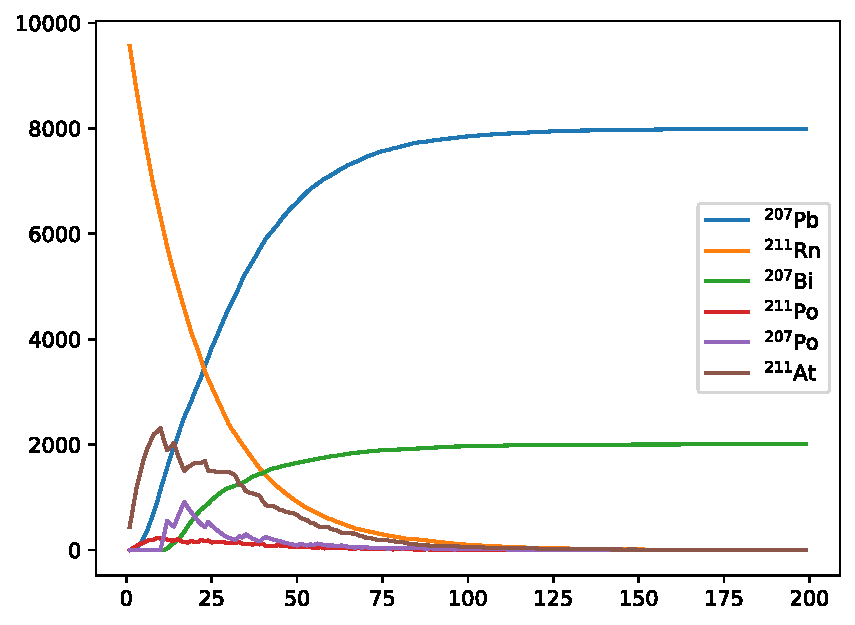
\includegraphics[width=\columnwidth]{02j_rn211_branching_decay_chain}
\caption{Branching chain starting from $10^4$ $^{211}$Rn nuclei, followed for $200$~h. The two end products $^{207}$Pb and $^{207}$Bi saturate in the $74:26$ ratio of the branch; the sawtooth in the intermediates reflects the once-per-step branching decision discussed in the text.}
\label{fig:branching}
\end{figure}

\section{Act III: Evolve}
\label{sec:evolve}

\subsection{A gas, one collision at a time}

The third act turns the random initial conditions of Act~II into deterministic dynamics. Two hundred molecules of mass $6.7\times10^{-27}$~kg (helium) are placed uniformly in a cube of half-side $L=1$~m at $T=300$~K, all with speed $v_{\rm th}=\sqrt{2k_BT/m}$ and random direction, and the simulation is event-driven in the manner of Alder and Wainwright~\cite{AlderWainwright1959}: for every molecule and every wall the time to impact is computed, the smallest is taken, all molecules are advanced by that time, the velocity component of the colliding molecule is reversed, and the momentum $2m|v_\perp|$ it hands to the wall is accumulated. The pressure follows from the total momentum transferred per unit time and wall area.

The notebook's printed pressures start at a few $10^{-19}$~Pa (two hundred atoms in a cubic metre is a very good vacuum) and then, after a few collisions, turn into a column of \texttt{inf}, while the cumulative estimate grows linearly with the collision count (Fig.~\ref{fig:gas}). The run was kept exactly as it happened. The cause is identified in Sec.~\ref{sec:outlook}; what matters for the story is that an event-driven scheme is only as good as its event detection, and that a single wrong branch can freeze the clock.

\begin{figure}[tb]
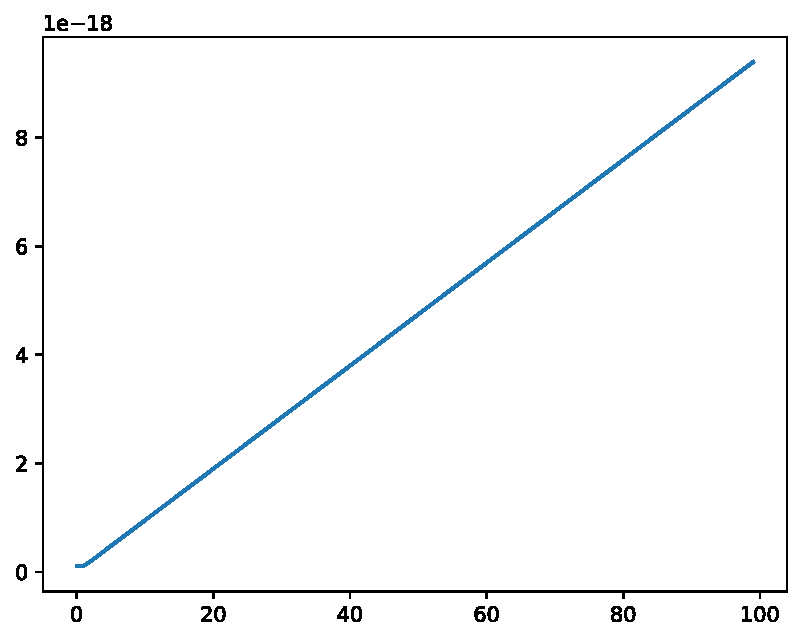
\includegraphics[width=\columnwidth]{03a_gas_pressure_vs_collisions}
\caption{Cumulative pressure estimate of the free-flight gas after each wall collision. The linear growth is an artefact: from the fourth collision on the simulation clock stops advancing while the momentum tally keeps growing (see Sec.~\ref{sec:outlook}).}
\label{fig:gas}
\end{figure}

\subsection{The heat equation three ways}

The course ends on a grid. The one-dimensional diffusion equation $u_t=\kappa u_{xx}$ on $[0,1]$ with $u(x,0)=\sin\pi x$ and $u=0$ at both ends has the exact solution $e^{-\pi^2\kappa t}\sin\pi x$, and three schemes were written for it with $\gamma=\Delta t/\Delta x^2$:
\begin{align}
\text{forward Euler:}&\quad u_i^{j+1}=\gamma u_{i+1}^{j}+(1-2\gamma)u_i^{j}+\gamma u_{i-1}^{j},\nonumber\\
\text{backward Euler:}&\quad A\,\mathbf u^{j+1}=\mathbf u^{j}+\mathbf b,\nonumber\\
\text{Crank--Nicolson:}&\quad A'\mathbf u^{j+1}=B'\mathbf u^{j}+\mathbf b',
\end{align}
with the tridiagonal matrices written out in the notebook~\cite{CrankNicolson1947,Crank1975}. The implicit schemes solve a $39\times39$ linear system per step with \texttt{numpy.linalg.solve}.

The grid chosen, $\Delta x=\Delta t=0.025$, gives $\gamma=40$. This is eighty times the stability limit $\gamma\le\tfrac12$ of the explicit scheme~\cite{CFL1928}, and Fig.~\ref{fig:heat} shows the consequence in one glance: the backward-Euler and Crank--Nicolson panels display the sine profile decaying smoothly, while the forward-Euler panel is a sawtooth with amplitude $10^{71}$ after forty steps. The third instructive failure is thus the most classical one in the subject, and the most clearly diagnosed: unconditional stability is exactly what the two implicit schemes buy with their linear solve, and Crank--Nicolson adds second-order accuracy in time on top.

\begin{figure}[tb]
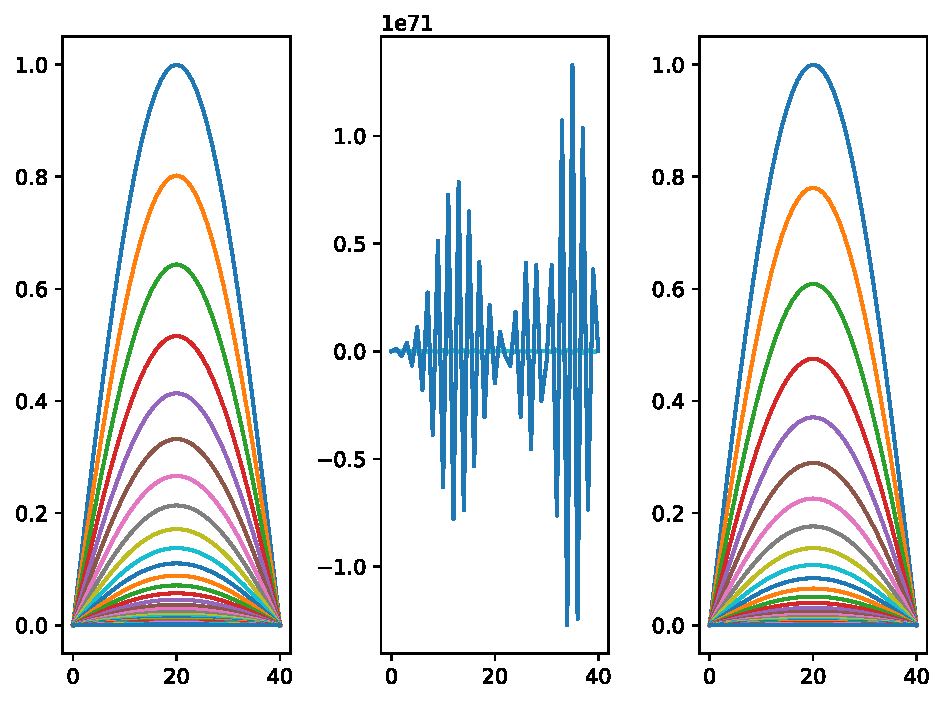
\includegraphics[width=\columnwidth]{03b_heat1d_implicit_explicit_crank_nicolson}
\caption{$u(x,t)$ for the 1-d heat equation with $u(x,0)=\sin\pi x$, $\Delta x=\Delta t=0.025$ ($\gamma=40$), one curve per time step. Left: backward Euler. Middle: forward Euler, unstable (note the $10^{71}$ scale). Right: Crank--Nicolson.}
\label{fig:heat}
\end{figure}

\section{Conclusion and outlook}
\label{sec:outlook}

Read as a whole, the repository is a record of one student acquiring the three reflexes of numerical physics. In Act~I the unknown is a fixed point and the computer walks towards it; the walk is fast when the update is Newton's and slow when it is the unshifted QR step, and in both cases the student had to decide when to stop. In Act~II the unknown is an average and the computer estimates it; the student discovered that the estimator matters (sample mean beats hit-or-miss), that the random numbers themselves have to be manufactured, that the error shrinks as $N^{-1/2}$, and that a few boolean arrays simulate a decay chain that is painful to solve on paper. In Act~III the unknown is a trajectory and the computer integrates it; the student met event-driven dynamics and the stability limit of explicit schemes.

The three failures are the natural outlook, because each has a one-line diagnosis that the author did not have at the time.

\paragraph{Eigenvectors.} Solving $(A-\lambda I)\mathbf v=\mathbf 0$ by any iteration started from $\mathbf 0$ returns $\mathbf 0$. The standard remedy is inverse iteration: start from a random vector, solve $(A-\lambda I)\mathbf v_{n+1}=\mathbf v_n$, normalise, repeat; because $A-\lambda I$ is nearly singular the component along the wanted eigenvector is amplified at every step. Alternatively the eigenvectors can be accumulated from the product of the $Q_k$ during the QR iteration itself.

\paragraph{The stalled gas.} After the global minimum collision time is found for molecule \texttt{mol}, the code decides which velocity component to reverse with a test that compares $t_x$ to $t_y$ and, only if $t_x\le t_y$, $t_x$ to $t_z$; when $t_y<t_x$ it reverses $v_y$ without ever looking at $t_z$. A molecule whose earliest impact is on a $z$-wall therefore reaches that wall with $v_z$ unchanged, sits exactly on it with $t_z=0$, and is selected again at every subsequent step with $t_{\rm col}=0$: the clock $T_n$ freezes at $1.1\times10^{-5}$~s (visible in the stored \texttt{tc} array), the division by $t_{\rm col}$ prints \texttt{inf}, and the cumulative pressure, $m\,\Delta V/(8LT_n)$ with $\Delta V$ still growing, rises linearly. A three-way minimum fixes it. Two smaller points for a future version: the $z$-velocity is built from $\cos\phi$ where $\cos\theta$ was intended, and all molecules share the same speed $v_{\rm th}$ rather than being drawn from the Maxwell--Boltzmann distribution that Act~II had just learned to sample.

\paragraph{The exploding heat equation.} Nothing is wrong with the code; $\gamma=40$ simply violates $\gamma\le\tfrac12$. Reducing $\Delta t$ to $2.5\times10^{-4}$ would make the explicit panel look like the other two, at the cost of a hundred times more steps---which is precisely the trade-off the implicit schemes exist to avoid.

\paragraph{Smaller items.} The Monte-Carlo decay curve would sit on the analytic one if the per-step survival were $e^{-p\Delta t}$ instead of $1-p\Delta t$, or if $\Delta t$ were made small; the branching chain would lose its sawtooth with a per-nucleus branch decision; the Box--Muller overlay has $\sigma^2$ on the wrong side of the fraction.

None of this will be fixed. The code is kept as it was written, by hand, as the last of its kind by this author, and the reorganised repository exists so that the story above can be followed by opening three notebooks in order.

\appendix

\section{Repository layout}
\label{app:repo}

\begin{description}
\item[\texttt{notebooks/}] the three acts: \texttt{01\_iterate}, \texttt{02\_sample}, \texttt{03\_evolve}. The prose is the original, word for word; the function bodies were moved out and are called from the notebooks.
\item[\texttt{compphys/}] those function bodies as an importable package, docstrings and comments intact, one module per topic.
\item[\texttt{figures/}] every plot produced during the course, named by content and indexed in a table.
\item[\texttt{literature/}] the primary references for each method, with DOIs, and the BibTeX file used by this note.
\item[\texttt{report/}] this note.
\item[\texttt{misc/}] the six original files, untouched, including the three stand-alone midterm scripts that duplicate the notebook.
\end{description}

\bibliography{../literature/references}

\end{document}
